\chapter{External Interfaces\label{sec:External-Interfaces}}


\section{Optimizing Through an External Command\label{sub:Optimizing-external-cmd}}

\begin{figure}
\noindent \begin{centering}
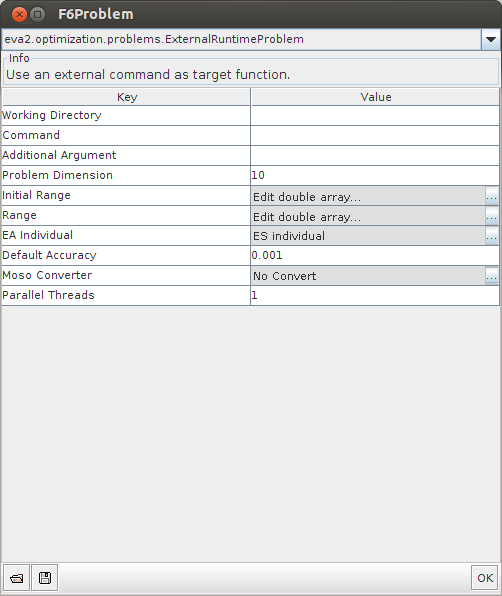
\includegraphics[width=0.4\columnwidth]{pics/screenshot-ExtRun}
\par\end{centering}

\caption{Screenshot of an external runtime problem configuration.\label{fig:Screenshot-external-runtime}}
\end{figure}


For easy optimization using a runnable program, we provide the \texttt{ExternalRuntimeProblem}
class. So if you have a runnable function implementation called ``\emph{testEval}''
(or ``\emph{testEval.exe}''), that takes a series of double valued
arguments and produces a result value as output (on \textit{stdout}),
you can select \texttt{ExternalRuntimeProblem} in the GUI, enter the
path and program name into the command field, adapt boundaries and
the problem dimension and just start optimization. For a programm
called \textit{testEval} with a two-dimensional solution space, which
you want to optimize within $[-5,10]^{2}$, the configuration can
be seen in Fig.~\ref{fig:Screenshot-external-runtime}. In the example,
\textit{testEval} may be called and, in the single objective case,
should produce output as in:
\begin{quotation}
\begin{flushleft}
\texttt{\$ /home/username/testEval 7.1642923 -4.2346211}
\par\end{flushleft}

\begin{flushleft}
\texttt{28.1371802}
\par\end{flushleft}

\begin{flushleft}
\texttt{\$ \_}
\par\end{flushleft}
\end{quotation}
\noun{EvA2} starts a system process to run the external program and
converts input/output using String objects, which is by itself rather
slow. Still, it may outweigh the costs of reimplementing it anew and
can even be negligible if the runtime of the calculation is of higher
order of magnitude. It may also just come in handy if you want to
try what \noun{EvA2} might do for you.


\section{Optimization from Matlab\label{sub:Optimization-from-Matlab}}


\subsection{Quick Howto\label{sub:JEInterface-Quick-Intro}}

To tackle optimization problems already existing in Matlab, we provide
a simple Matlab interface comprising in a Matlab class definition.
The Matlab m-files are located in the EvA2 resources folder of the
distributed binary jar or can be downloaded from the homepage. If
you have an existing Matlab function you want to optimize with some
standard algorithms implemented in \noun{EvA2}, you can do this directly
from your Matlab console. 

A Matlab function, e.g., \texttt{testfun.m} , as in Alg.~\ref{alg:Example-m-function}
will be used to repeatedly evaluate candidate solutions. Three basic
data types are designated for use with the Matlab interface, denoted
by flags \texttt{'binary'}, \texttt{'int'}, or \texttt{'double'}.
Depending on the data type flag, a binary, integer, or real-valued
individual type will be used. The matlab function will receive a char
of symbols '0'/'1' or an integer array or a double array, respectively. 

To run an optimization from Matlab, look at the following steps. For
explicit examples, look at Algs.~\ref{alg:Optimization-from-Matlab-integer}-\ref{alg:Optimization-from-Matlab-int.}
and the exemplary target function listed in Alg.~\ref{alg:Example-m-function}.
\begin{enumerate}
\item Download the EvA2.jar and add it to the Matlab classpath, e.g.
by typing \texttt{javaaddpath '/home/username/EvA2.jar'} in the
Matlab console.
\item Extract the Matlab JEInterface code to your Matlab working directory
within its own class directory ``@JEInterface''.
\item Define the range of your search space using a $2\times d$ matrix
consisting of the lower and upper bounds of the allowed space, e.g.
enter \texttt{R={[}-5 -5 -5;5 5 5{]}} to define a 3-dimensional real
valued search space with bounds -5/5 in each dimension. For binary
problems, \texttt{R} should be a positive integer, e.g., \texttt{R=20}
for a binary problem with 20 bits.
\item For a target function \texttt{testfun.m} to be minimized, create a
JEInterface in Matlab by typing, for example: \texttt{JI=JEInterface(@testfun,
'double', R)}. Notice that \texttt{testfun.m} must be accessible from
your working directory, it should not be placed in the @JEInterface
directory. For integer or binary target functions, replace '\texttt{double'}
by \texttt{'int'} or \texttt{'binary'}, respectively.
\item To view the possible optimization strategies, type \texttt{showOptimizers(JI)}.
\item You can now select an optimizer and use its ID to start the optimization,
e.g. \texttt{JI=op\-ti\-mize\-(JI,1)} for a standard ES.
\item Wait for the optimization to finish and type \texttt{getResult(JI)}
to get the best solution found.
\end{enumerate}

\subsection{Details on JEInterface}

The main \texttt{optimize} command actually starts two new Java threads
handling Java callbacks to Matlab within the single Matlab thread.
The result of the optimization will be written back to the JEInterface
instance and is not a direct output value of the \texttt{optimize}
call. There will be a text notice in the Matlab console as soon as
the optimization has finished. Notice that in Matlab object oriented
style, an object \texttt{Obj} cannot be modified simply by calling
the mutator, e.g. \texttt{setOpt(Obj, p1, val1)}, but must be reassigned
for every mutating call, as in: \texttt{Obj=setOpt(Obj, p1, val1)}.
After optimization, you may retrieve the result by calling \texttt{getResult}
on the interface instance. Or, in case you want to retrieve multiple
solutions to the target function, you may start a post processing
step and retrieve a list of solutions using \texttt{getMultipleSolutions}.

Some optimizers allow the solutions to get worse during the optimization
run. This allows them to overcome local optima and increases the chance
to find a global one. But on the other hand it means that the result
of the last optimization iteration is not necessarily the best solution
found during the whole run. Therefore, \noun{EvA2} saves the best
solution found external to the optimizer, which is what is returned
by the \texttt{getResult} method. 

Most optimization strategies have specific parameters influencing
their performance. The \texttt{optimize}-call gives access to standard
parameter settings. To modify specific parameters, use the \texttt{getDesc}-method
to list available parameters of an optimizer. You may then use the
method \texttt{optimizeWith} and deliver specific parameters in name/value
pairs to configure a specific run, where the names must correspond
to a member variable of the optimizer as listed by \texttt{getDesc}
and the value object must of course be of the correct type.

\begin{algorithm}
\begin{mylstenv}
function z = testfun(x, y) 
switch y     
  case 1 % modulated parabola         
    z(1)=sum(x.*x)+cos(x(1))*sin(x(2));     
  case 2 % Branin         
    z(1)=(x(2)-(5/(4*pi^2))*x(1)^2+5*x(1)/pi-6)^2+10*(1-1/(8*pi))*cos(x(1))+10;     
  case 3 % Himmelblau         
    z(1)=((x(1)^2 + x(2) - 11)^2 + (x(1) + x(2)^2 - 7)^2);     
  case 4 % simple binary, minimize bits
    z(1)=0;
    for i=1:length(x)          
      if (x(i)=='1') ; z(1)=z(1)+1; end         
    end     
  case 5 % simple parabola         
    z(1)=sum(x.*x);
end
\end{mylstenv}

\caption{Example m-function for optimization from Matlab\label{alg:Example-m-function}}
\end{algorithm}


For further details, check the method overview in the list below.
Each interface method (except the constructor) has at least a parameter
\texttt{JI}, designating the JEInterface object to work on.
\begin{description}
\item [{\texttt{JI=JEInterface(fHndl,datatype,R,{[}initR{[},fArg{[},optName,optValue{]}{*}{]}{]})}}] JEInterface
constructor: \emph{fHndl}: handle of the target function. \emph{datatype}:
give a char 'int', 'binary', or 'double' depending on the desired
data type. \emph{R}: a 2$\times$dim array defining the solution subspace
with lower and upper bounds. \emph{initR}: For the integer and real
valued case, an initialization range can optionally be set, but must
be a subset of \emph{R} of same dimensions -- often it can be set
equal to \emph{R}. \emph{fArg}: additional static parameters to the
target function as single object (scalar, struct, or list). \emph{optName,
optValue}: optional name-value pairs defining \emph{MaxFunCalls},
\emph{TolX} and \emph{TolFun} similar to the Matlab optimset structure.
The \emph{Display} option may trigger verbose output. 
\item [{\texttt{showOptimizers(JI)}}] Print a list of optimization strategies
accessible through JEInterface by ID numbers.
\item [{\texttt{JI=optimize(JI,optType{[},resultFilePrefix{]})}}] Start
the optimization using the strategy indicated by the ID \emph{optType}.
Optionally write verbose results to an output file with prefix \emph{resultFilePrefix}
in the working directory. Returns the modified JEInterface instance.
The method also opens a message box with a cancel button to stop the
optimization.
\item [{\texttt{{[}sol,fit{]}=getResult(JI)}}] After optimization: return
the final solution and its fitness. During optimization: return the
current best solution and its fitness.
\item [{\texttt{getMessage(JI)}}] Return a text message describing the
termination state of the optimization, e.g. the number of function
calls performed.
\item [{\texttt{JI=postProcess(JI,steps,sigmaClust{[},nBest{]})}}] Do post-processing
of the last optimization results and export the solution set to the
interface instance (cf. Sec.~\ref{sub:Post-Processing}). If \emph{sigmaClust}
> 0 a clustering step is performed (density based clustering), so
that any solutions in a distance below \emph{sigmaClust} are associated.
Notice that \emph{sigmaClust} is treated relative to the problem range.
If \emph{steps} > 0, then a hill climbing step is performed after
clustering for the given number of evaluations. If \emph{nBest} is
given, it defines the maximal number of solutions to be exported to
the interface instance. Post processing can be stopped by \texttt{JI=stopOptimize(JI)}
just as the optimization itself.
\item [{\texttt{{[}sols,fits{]}=getMultipleResults(JI)}}] After optimization
or post-processing: retrieve the solution set in a matrix and calculate
the corresponding fitness values.
\item [{\texttt{makeOptions(JI{[},optName,optVal{]}{*})}}] Produce an options
structure with given settings. Notice that you need to use setOptions
with the returned structure to apply the options for a given JI instance,
as in: \texttt{JI=setOptions(JI,makeOptions(JI,'TolX',1e-8))}. 
\item [{\texttt{getOptions(JI)}}] Get the current \emph{optimset} structure
of the JEInterface instance.
\item [{\texttt{getOpt(JI,optName)}}] Get the value of a specific option
\emph{optName} from the \emph{optimset} structure of the JEInterface
instance.
\item [{\texttt{JI=setOpt(JI,optName,optVal)}}] Set a specific option \emph{optName}
of the \emph{optimset} structure in \texttt{JI} to the value \emph{optVal}.
Returns the modified JEInterface instance.
\item [{\texttt{JI=setOptions(JI,optset)}}] Set a whole new \emph{optimset}
structure \emph{optset}. Returns the modified JEInterface instance.
\item [{\texttt{getDesc(JI,optTypeOrObject{[},showValues{]})}}] Show information
about an optimizer class (if \texttt{optType} is an integer ID) or
any other object together with the parameters that can be modified
in a standardized way. The available settings are analogous to the
optimizer options presented by the Java GUI. If \texttt{showValues==1}
holds, the current values of the given instance are displayed as well.
\item [{\texttt{optimizeWith(JI,optType{[},outputFilePrefix{]}{[},memName,memVal{]}{*})}}] Optimize
using an optimizer by ID and specific settings for this optimizer.
The settings given must conform to the options shown by \texttt{getDesc(JI,optType)}.
The available settings are analogous to the optimizer options presented
by the Java GUI. The method also opens a message box with a cancel
button to stop the optimization.
\item [{\texttt{testEvalFunc(JI)}}] Test the function handle for some basic
conformations with expected output.
\item [{\texttt{setVerbose(JI,swtch{[},fname{]})}}] Activate debug output
if \emph{swtch} is 1, else deactivate it. If \emph{fname} is given,
that's the filename the debug information is written to.
\item [{\texttt{JI=stopOptimize(JI{[},'kill'{]})}}] Stop a running optimization
process, which is usually done by the cancel button. In case brute
force was used (STRG-C), this method may be used with the \texttt{'kill'}
argument to try to clean up Java threads still running as ``zombies''.
\item [{\texttt{setResultJE}}] (Internal) Write-back method required internally
by \noun{EvA2}. Calling it by hand may interfere with optimization.
\item [{\texttt{setResultArrayJE}}] (Internal) Write-back method required
internally by \noun{EvA2}. Calling it by hand may interfere with optimization.
\item [{\texttt{getProgress(JI)}}] (Internal) During optimization, return
the number of fitness calls performed until now.
\item [{\texttt{runEvalLoopJE}}] (Internal) Start a EvA run, optimization
or post processing.
\end{description}
The methods are listed in about the order a user might require them
in. The constructor as well as all mutating methods return a JEInterface
object which is to be assigned to a variable, preferably the same
as the one assigned on construction. This is a drawback of the Matlab
object concept: mutators are actually also constructors and copy the
whole Matlab object, but they do not copy the referenced Java instance.
Notice that the last three methods, \texttt{setResultJE}, \texttt{setResultArrayJE}
and \texttt{evaluateJE}, are used internally by the Java part of the
interface and should not be called by hand. To find out more about
the optimization strategies you can access through JEInterface, use
the \texttt{showOptimizers} method and take a look at the EA references,
e.g. the technical report on \noun{JavaEvA} \cite{JOptDocumentation}. 

\begin{table}
\begin{tabular}{|c|c|c|}
\hline 
{\footnotesize Option name} & {\footnotesize Values} & {\footnotesize Description}\tabularnewline
\hline 
\hline 
{\footnotesize Display} & {\footnotesize 'off' | 'iter' | 'final' | 'notify'} & {\footnotesize Output verbosity to Matlab console.}\tabularnewline
{\footnotesize MaxFunEvals} & {\footnotesize positive integer} & {\footnotesize Maximum number of evaluations to be performed.}\tabularnewline
{\footnotesize MaxIter} & {\footnotesize --} & \emph{\footnotesize Unused}{\footnotesize .}\tabularnewline
{\footnotesize TolFun} & {\footnotesize real} & {\footnotesize Absolute convergence bound in function codomain.}\tabularnewline
{\footnotesize TolFunEvals} & {\footnotesize positive integer} & {\footnotesize No. of evaluations of the TolFun convergence criterion.}\tabularnewline
{\footnotesize TolX} & {\footnotesize real} & {\footnotesize Absolute convergence bound in function domain.}\tabularnewline
{\footnotesize TolXEvals} & {\footnotesize positive integer} & {\footnotesize No. of evaluations of the TolX convergence criterion.}\tabularnewline
\hline 
\end{tabular}

\caption{JEInterface optimization options overview.\label{tab:JEInterface-optimization-options.}}
\end{table}



\subsection{Optimization Options}

Vital for the usage in Matlab are the termination criteria of the
optimization run. We adopt some parameters from the builtin \emph{optimset}
structure in analogy to the Matlab function \emph{fminsearch}. To
find out more about \emph{optimset}, check the Matlab documentation.
The JEInterface options provided are listed in Tab.~\ref{tab:JEInterface-optimization-options.}.
Display triggers output to the Matlab console during an optimization
process. While \texttt{'final'} only shows final optimization results,
'\texttt{notify}' corresponds to ``show every k-th iteration'' while
'\texttt{iter}' corresponds to ``show all iterations'' compared
to the GUI options. The default is '\texttt{off}'. An optimization
run terminates if MaxFunEvals has been reached or the best solution
changes both in domain and codomain less than TolX and TolFun for
a certain number of evaluations, which may be set using TolXEvals
and TolFunEvals, respectively. If TolX is positive, the run is seen
as converged, if the best individual (the best parameter set) does
not change more than the threshold defined by TolX for a number of
TolFunEvals evaluations. Convergence in the fitness domain is defined
in the same way using TolFun and TolFunEvals. 

If no options are defined through the constructor, the default values
for \emph{TolX} and \emph{TolFun} are the same as in Matlab ($10^{-4}$),
while the default value for \emph{MaxFunEvals} is usually $10^{4}$.
You can check the options by calling \emph{getOptions} for a JEInterface
instance. In analogy to \emph{fminsearch}, the three criteria will
be logically combined as in $(MaxFunEvals\;\mathrm{OR}\;(TolX\;\mathrm{AND}\; TolFun))$,
meaning that reaching \emph{MaxFunEvals} is a hard stopping criterium,
while \emph{TolX}/\emph{TolFun} must be both fulfilled to stop the
run, if \emph{MaxFunEvals} has not been reached. To change options
on an existing object \texttt{JI}, call for example \texttt{JI=setOpt(JI,
'TolFun', 1e-7)} to set the TolFun convergence threshold to $10^{-7}$.
If you don't want to regard convergence and just have the optimization
perform a certain number of evaluations, set \emph{TolX} and \emph{TolFun}
to zero, e.g. by typing \texttt{JI=setOptions(JI, makeOptions(JI,
'TolX', 0, 'TolFun', 0))}. To perform not more than $10^{5}$ and
stop earlier if the best solution's fitness has not changed by more
than 0.1 for 1000 evaluations, set MaxFunEvals=$10^{5}$, TolX=0,
TolFun=0.1 and TolFunEvals=1000. Be aware that at least one termination
criterion must be defined through the options, or the optimization
will not start. 


\subsection{Usage Example}

Listing~\ref{alg:Example-m-function} shows an exemplary m-File that
could be used as target function in an optimization through Matlab.
Notice that the paramter \emph{y} might be used in any other way or
not used at all. \noun{EvA2} will not introspect the contents of \emph{y},
but just hand it over to every call to the target function where it
may be assumed static. So to optimize the Himmelblau function using
Particle Swarm Optimization, proceed in the Matlab console as shown
in Listing~\ref{alg:Optimization-from-Matlab-integer}. For a binary
optimization, you might set \texttt{R=50}, for example, the target
function will then receive 2 uint32's of which 50 bits are to be used
in the target function. 

\begin{algorithm}
\begin{mylstenv}
javaaddpath '/home/username/workspace/EvA2.jar'
initR=[-15 -15 -15 -15 -15; -5 -5 -5 -5 -5]; 
R=[-15 -15 -15 -15 -15; 15 15 15 15 15]; 
JI=JEInterface(@testfun, 'int', R, initR, 5, 'Display', 'iter');  % "5" indicates parabola
JI=optimize(JI, 3);  % starts a Genetic Algorithm with integer-based individuals
[sol, fit]=getResult(JI); 
\end{mylstenv}

\caption{Optimization from the Matlab console, integer example with specific
initialization range.\label{alg:Optimization-from-Matlab-integer}}
\end{algorithm}


\begin{algorithm}
\begin{mylstenv}
javaaddpath '/home/username/workspace/EvA2.jar'
R=20; 
JI=JEInterface(@testfun, 'binary', R, R, 4, 'Display', 'iter'); % "4" indicates minimize bits
JI=optimize(JI, 3);  % start a default Genetic Algorithm
[sol, fit]=getResult(JI); 
[finalPop, finalFit]=getMultipleResults(JI);
\end{mylstenv}

\caption{Optimization from the Matlab console, binary example.\label{alg:Optimization-from-Matlab-binary}}
\end{algorithm}


\begin{algorithm}
\begin{mylstenv}
javaaddpath '/home/username/workspace/EvA2.jar'
R=[-5 -5 -5; 5 5 5];
JI=JEInterface(@testfun, 'double', R, R, 1, 'Display', 'iter', 'TolX', 0, 'TolFun', 0); 
JI=optimize(JI, 4);  % starts a default Particle Swarm Optimization run
[sol, solFit]=getResult(JI);
\end{mylstenv}

\caption{Optimization from the Matlab console, real-valued example.\label{alg:Optimization-from-Matlab-int.}}
\end{algorithm}
